%!TEX root = ../schoedon.tex

\cleardoublepage
\chapter{Overview and related work}
  \label{chap:overv}

  Table \ref{tab:overv:relat} (page \pageref{tab:overv:relat}) shows a first
  overview of related graphics, applications and publications in the broad
  field of mobility analytics and accessibility mapping techniques.\par

  \begin{table}[htp]
    \tiny \centering
    \begin{tabular}{r|l|l|l}
     \textbf{Year} & \textbf{Authors} & \textbf{Contribution} & \textbf{Type} \\
     \hline
      1881 & Galton \cite{galton1881construction} & Construction of isochronic passage-charts  & Publication  \\
      1959 & Hansen \cite{hansen1959accessibility} & How accessibility shapes land use & Publication \\
      1972 & Armstrong \cite{armstrong1972network} & Network analysis of airport accessibility  & Publication  \\
      1978 & Muller \cite{muller1978mapping} & Mapping of travel times  & Publication  \\
      1981 & Sugiura \cite{Sugiura1981} & Japan travel time maps  & Graphic  \\
      1986 & Hall \cite{hall1986fastest} & Network with random time-dependent travel times  &  Publication \\
      1989 & Cauvin et al. \cite{cauvin1989cartographic} & The piezopleth maps method  & Publication  \\
      1993 & Spierkermann et al. \cite{spiekermann1993zeitkarten} & Time maps for spatial planning  & Publication  \\
      1994 & Spierkermann et al. \cite{spiekermann1994new} & Time-space maps of Europe  & Publication  \\
      1996 & Gutierrez et al. \cite{gutierrez1996accessibility} & Accessibility analysis of the European road network  & Publication  \\
      1998 & Fritz et al. \cite{fritz1998accessibility} &  Accessibility as wilderness indicator  & Publication  \\
      1999 & Spiekermann \cite{spiekermann1999visualisierung} & Visualization of railway travel times & Publication \\
      2000 & Miller et al. \cite{miller2000gis} & GIS for measuring space-time accessibility in transportation & Publication \\
      2000 & O'Sullivan et al. \cite{o2000using} & Using desktop GIS for accessibility analysis in public transport  & Publication  \\
      2001 & Ran \cite{ran2001method} &  Method of providing travel time  & Patent \\
      2001 & Handy \cite{handy2002accessibility} & Accessibility versus mobility & Publication \\
      2002 & Lovett et al. \cite{lovett2002car} & Accessibility of general practitioner services  & Publication  \\
      2003 & Dailey et al. \cite{dailey2003design} &  Multi-modal transit management system & Publication  \\
      2005 & Auxhausen \cite{axhausen2005zeitkarten} & Time-maps of Switzerland  & Publication  \\
      2005 & Chronomap \cite{Chronomap} & Drive-time analysis  & Application  \\
      2005 & Karlin \cite{Karlin2005}  & London subway travel times  & Graphic \\
      2005 & McLaren \cite{McLaren2005} & Time travel with the London tube map  & Graphic  \\
      2005 & Travel Time Tube Map \cite{Carden2006} & Interactive travel time tube map  & Application  \\
      2006 & Lightfoot \cite{Lightfoot2006} & Use-cases for travel time maps  &  Publication  \\
      2006 & Pfoser et al. \cite{pfoser2006dynamic} &  Dynamic travel time maps & Publication  \\
      2006 & Rüegg \cite{Ruegg2006} & Impact of public transport on travel times  & Poster \\
      2006 & Street \cite{street2006timecontours} & Isochrone visualization to describe transport network costs  & Master's Thesis  \\
      2007 & Irving \cite{Irving2007} & Use-cases for travel time maps  & Publication  \\
      2007 & Nies et al. \cite{neis2007webbasierte} & Web-based accessibility analysis  & Publication  \\
      2008 & Bauer et al. \cite{bauer2008computing} & Isochrones in multi-modal transportation networks  & Publication  \\
      2008 & Mapumental \cite{Mapumental}  &  Maps that show time & Application  \\
      2008 & Uchida et al. \cite{Uchida2008} & Travel time to major cities  & Graphic  \\
      2009 & FreeMapTools \cite{Freemaptools} & How far can I travel  & Application  \\
      2009 & Uchida et al. \cite{uchida2009agglomeration} & Measure of urban concentration  & Publication  \\
      2010 & Antrim et al. \cite{antrim2013many} & Use-cases for GTFS data & Publication  \\
      2010 & Campenhout \cite{van2010travel} & Travel time maps  & Master's Thesis  \\
      2010 & Glander et al. \cite{Glander2010} & Accessibility maps to visualize quality of mobility  &  Publication \\
      2010 & Lei et al. \cite{lei2010mapping} & Mapping transit-based access  & Publication  \\
      2010 & Marciuska et al. \cite{marciuska2010determining} & determining objects within isochrones  & Publication  \\
      2010 & Müller et al. \cite{Mueller2010} & Distance transformations for accessibility mapping  &  Publication \\
      2010 & Time Maps \cite{TimeMaps} & Public transport time maps of the Netherlands & Application  \\
      2011 & Birchler \cite{birchler2011computing} & Isochrones in multi-modal public transport networks  & Bachelor's Thesis  \\
      2011 & Gemmel \cite{gemmel2012hedonic} &  Effects of walk-ability and public transit & Master's Thesis  \\
      2011 & Gamper et al. \cite{gamper2011defining} & Defining isochrones in multi-modal spatial Networks & Publication  \\
      2011 & Isochrone.ch \cite{IsochroneCh}  & Isochrones in schedule-based public transport  & Application  \\
      2011 & Li et al. \cite{li2011dynamic} & Dynamic accessibility mapping  & Publication  \\
      2011 & Söderström \cite{soderstrom2011personal} & Internet-driven maps based on time distances  & Publication  \\
      2012 & Byrd \cite{Byrd2012} & Visualizing urban accessibility  & Publication  \\
      2012 & Gamper et al. \cite{gamper2012scalable} & Computation of isochrones with network expiration  & Publication  \\
      2012 & Conveyal \cite{Conveyal} & Transportation - land use analysis  & Application  \\
      2012 & Hollburg et al. \cite{hollburghier} & Interactive accessibility analysis in Potsdam & Publication  \\
      2012 & Mapnificent \cite{Mapnificent}  & Web-based reachability visualization of public transport  & Application  \\
      2012 & Mertens \cite{meertens2012} & Travel Time Maps of urban areas in the Netherlands  & Graphic  \\
      2012 & TripTropNYC \cite{TriptropNYC} & Web-based accessibility visualization in New York  & Application  \\
      2013 & Innerebner \cite{Innerebner2013} & Isochrones in multi-modal spatial networks  & PhD Thesis  \\
      2013 & Innerebner et al. \cite{innerebner2013isoga} & Web-based geospatial reachability analysis tool  & Publication  \\
      2013 & Transit Time NYC \cite{TransitTimeNYC} & Web-based subway transit times in New York & Application \\
      2013 & Tran et al. \cite{tran2013go_sync} & Synchronizing transit data between GTFS and OSM  & Publication  \\
      2014 & Gortana et al. \cite{gortanaisoscope} & Visualizing temporal mobility variance  & Publication  \\
      2014 & Hollburg \cite{Hollburg2014} & Interactive analysis and visualization of accessibility & Master's Thesis  \\
      2014 & Isoscope \cite{Isoscope} & Visualizing mobility with isochrone maps  & Application  \\
      2014 & Route360° \cite{Route360} & Web-based travel time analysis  & Application  \\
      2014 & Krismer et al. \cite{krismer2014incremental} & Incremental calculation of isochrones  & Publication  \\
      2014 & Voll \cite{vollerreichbarkeiten} & Accessibility analysis of the Alps  & Publication  \\
      2015 & TravelTimePlatform \cite{TravelTimePlatform} & Search and filter by time not distance  & Application  \\
      2015 & Yin et al. \cite{Yin2015} & Web-based accessibility analysis and travel time displays  & Publication  \\
      2016 & Schoedon et al. \cite{STHD2016} & Web-based visualization of transportation networks  & Publication  \\
    \end{tabular}
    \caption{Selected related work.}
    \label{tab:overv:relat}
  \end{table}

  \section{Noteworthy publications and theses}
    \label{sec:overv:publc}

    \begin{figure}[ht]
      \subcaptionbox{
        \label{fig:overv:isopc}
        The Isochronic Passage Chart by Francis Galton, 1881
        \cite{galton1881construction}.}
      {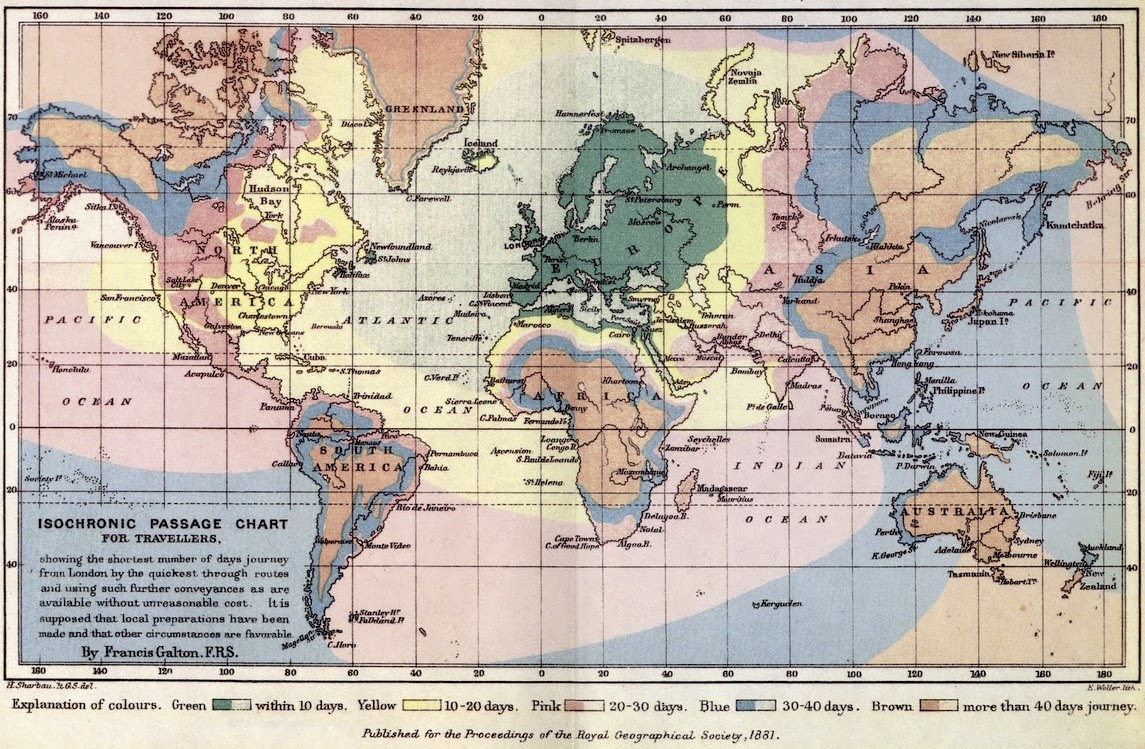
\includegraphics[width=0.32\textwidth]{./img/overv-isopc.jpg}}
      \hfill
      \subcaptionbox{
        \label{fig:overv:nodac}
        Analysis of Airport Accessibility in South Hampshire, 1972
        \cite{armstrong1972network}.}
      {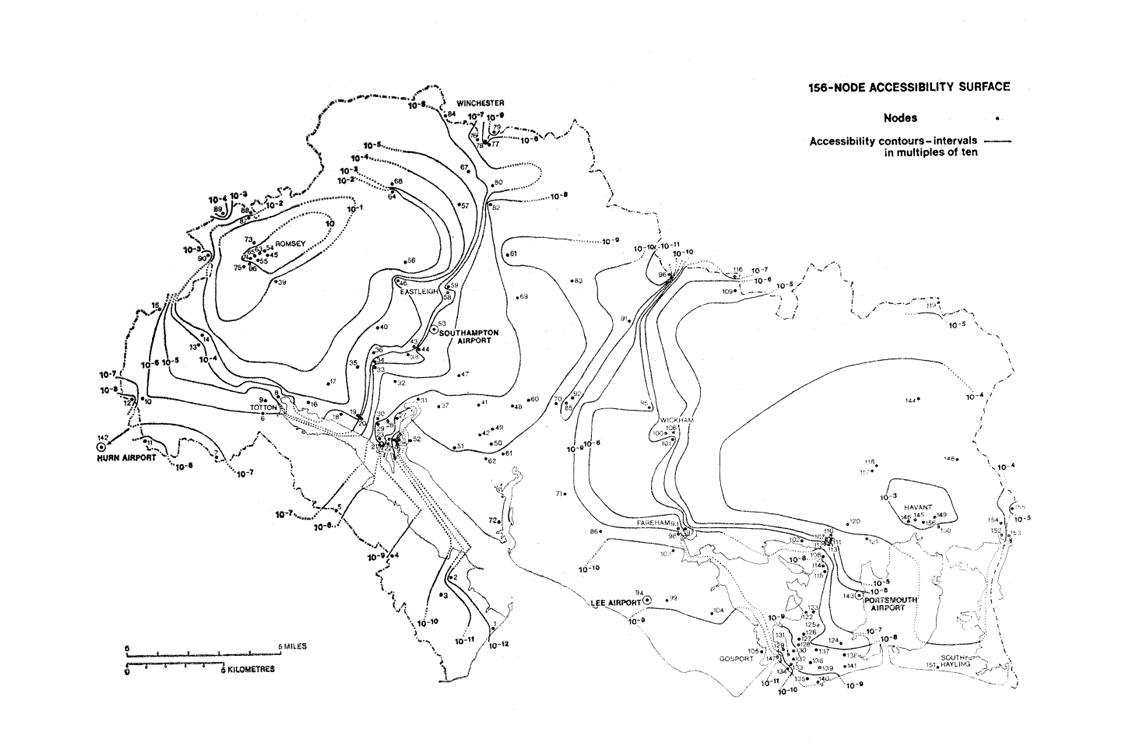
\includegraphics[width=0.32\textwidth]{./img/overv-nodac.png}}
      \hfill
      \subcaptionbox{
        \label{fig:overv:maptt}
        The Mapping of Travel Time in Edmonton, Alberta, 1978
        \cite{muller1978mapping}.}
      {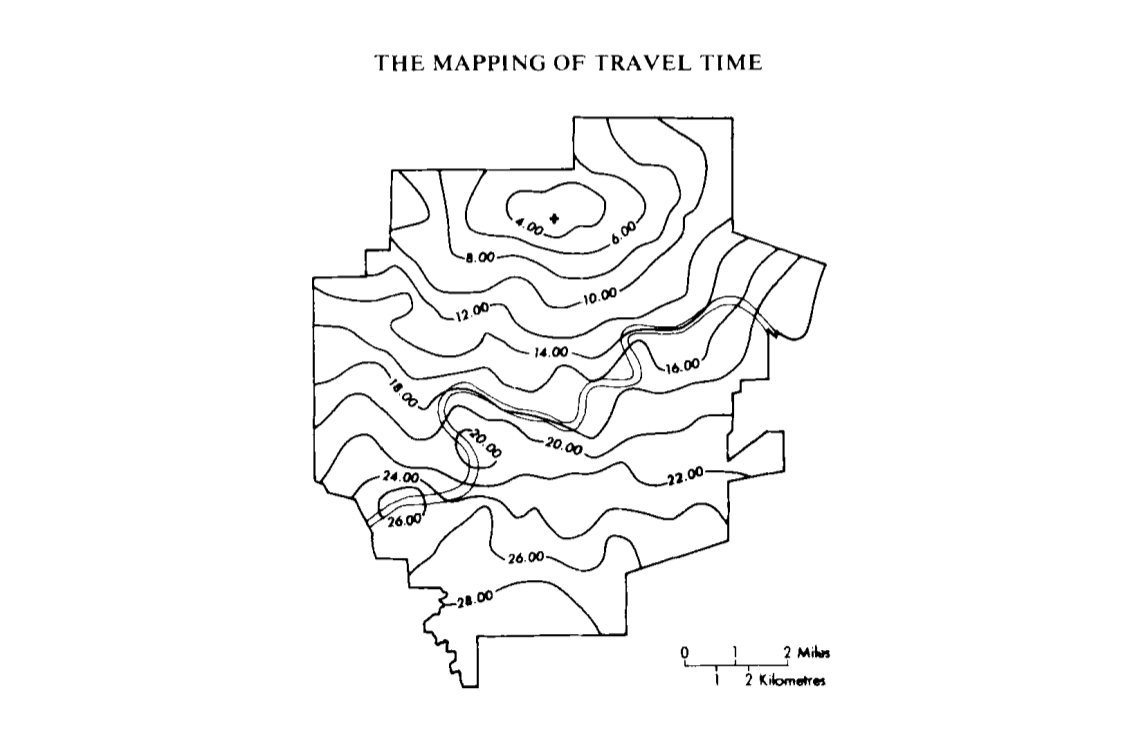
\includegraphics[width=0.32\textwidth]{./img/overv-maptt.png}}
      \label{fig:overv:1}
    \end{figure}

    In 1881 Francis Galton constructs the first isochronic map for the Royal
    Geographic Society (figure \ref{fig:overv:isopc}). It depicts the
    distances that can be traversed in equal times starting from London
    \cite{galton1881construction}. His contribution offers merely an isochronic
    generalization and suggests that future maps can be easily constructed for
    more detailled continental travel or home excursion maps.\par

    Among the first to define accessibility as indicator for urban
    transportation systems is Walter G. Hansen (1959). He presents a method for
    determining accessibility patterns within metropolian areas and defines
    accessibility as the potential of opportunities for interaction serving
    residents in urban areas \cite{hansen1959accessibility}.\par

    % armstrong 1972
    % transport costs play an important role
    % here: economic evaluation of airports
    % road travel times and weighting by importance for the application and population
    %%% GRAPHIC FIG 3or4

    Pioneer in computing accessibility analysis on the foundation of
    transportation networks is Harvey W. Armstrong (1972) who converted an
    exemplary road network with 159 nodes to a matrix and used a C.D.C. 6000
    computer to evaluate economic feasibility of airports in South Hamphsire
    \cite{armstrong1972network} (figure \ref{fig:overv:nodac}).\par

    Jean-Claude Muller (1978) highlights issues with the mapping of
    time-distances as the derived space is often non-euclidean and hardly
    mappable without distorting the geographic reference system
    \cite{muller1978mapping}. He presents a numerical approach for time-distance
    transformations of Edmonton and analysis the resulting distortions (figure
    \ref{fig:overv:maptt}).\par

    \begin{figure}[ht]
      \subcaptionbox{
        \label{fig:overv:patnt}
        Method of Providing Travel Time, 2001
        \cite{ran2001method}.}
      {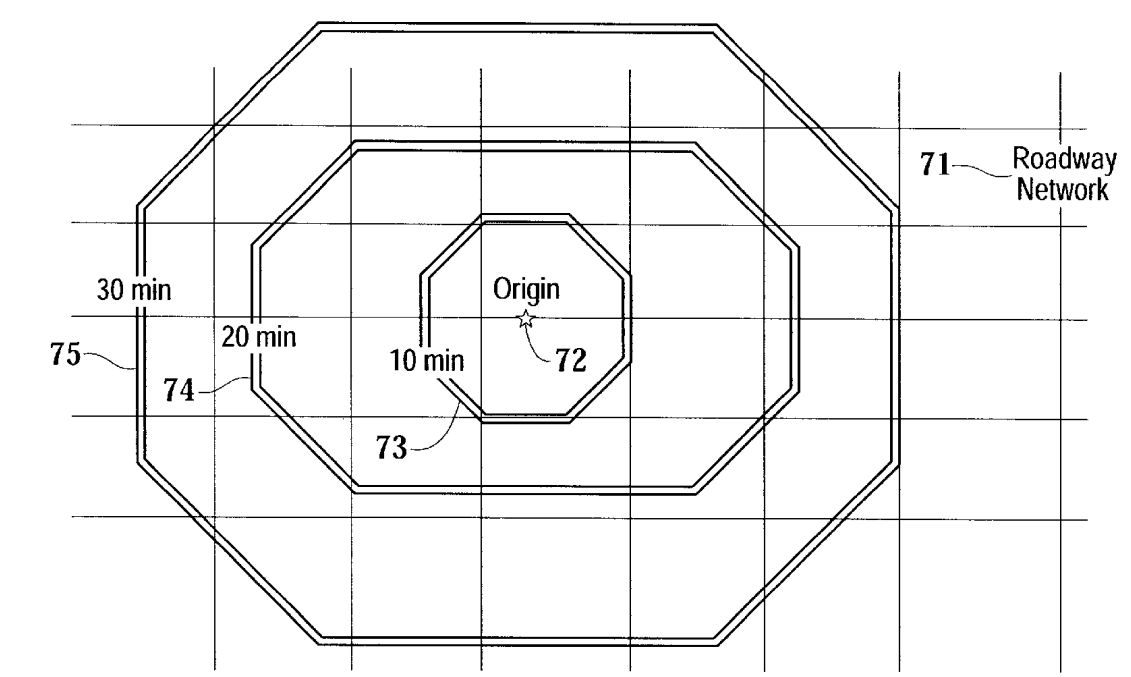
\includegraphics[width=0.32\textwidth]{./img/overv-patnt.png}}
      \hfill
      \subcaptionbox{
        \label{fig:overv:berln}
        Visualization of Quality of Mobility in Public Transport, 2010
        \cite{Glander2010}.}
      {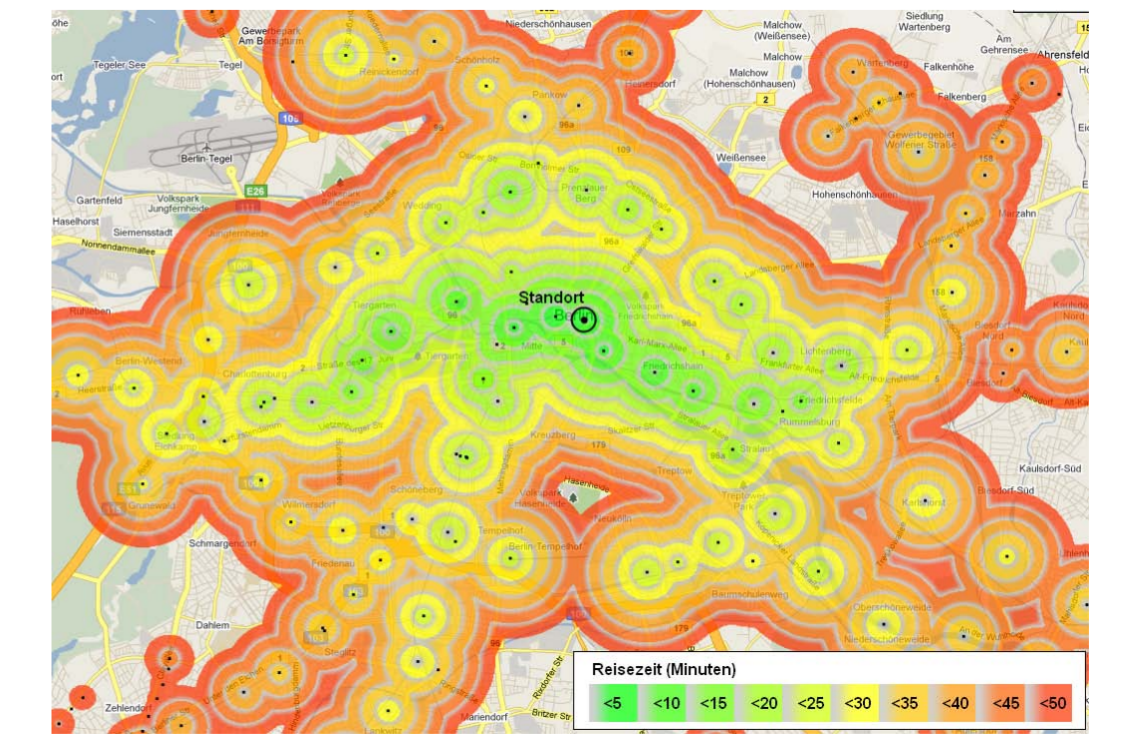
\includegraphics[width=0.32\textwidth]{./img/overv-berln.png}}
      \hfill
      \subcaptionbox{
        \label{fig:overv:potsd}
        Network-Based Accessibility Visualization in Potsdam, 2012
        \cite{hollburghier,Hollburg2014}.}
      {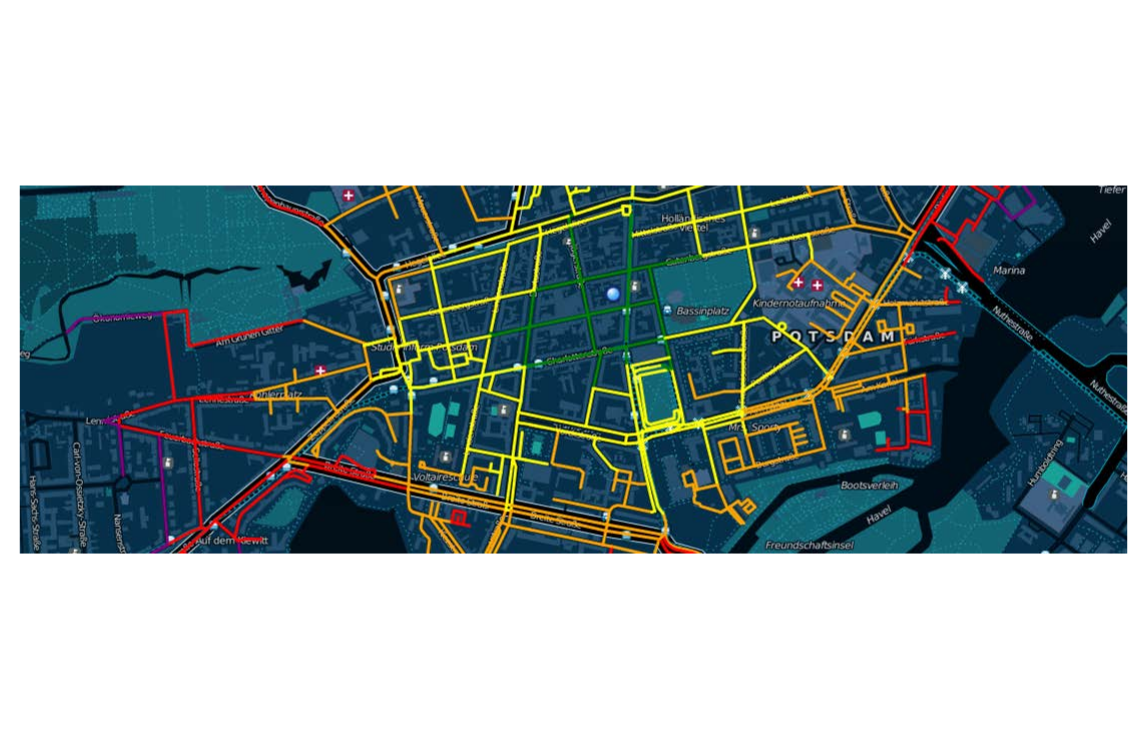
\includegraphics[width=0.32\textwidth]{./img/overv-potsd.png}}
      \caption{Shoo bar.}
      \label{fig:overv:2}
    \end{figure}

    The United States Patent and Trademark Office (\acrshort{uspto}) publishes
    the patent \#US006317686B1 issued by Bin Ran in 2001 on the method of
    providing travel time \cite{ran2001method}. It claims a personalized
    multi-modal travel prediction and trip decision support system including
    traffic forecast maps such as travel speed maps, travel time maps, and
    travel cost maps. It uses contour lines to represent predictive minimal
    travel time from a selected origin (figure \ref{fig:overv:patnt}).\par

    % street theis 2006
    % time based maps describe time accessibility of networks
    %%% FIG: 56 or 57 global integration of london (axial map) of network

    An important milestone and often cited reference is the final report on
    TimeContours by Nicholas Street (2006). It provides a Java application which
    maps isochrones onto public transport and road graphs to display
    transportation costs with respect to the travel time required
    \cite{street2006timecontours}. It discusses methods to display more than two
    dimensions on geographic maps such as isolines and defines isochrones --
    isolines of same time -- as derivation of the more commonly used isohypses
    -- isolines of the same height -- in a similar manner.\par

    % neis et al. 2007
    % utilizes attributed street network graph
    %%% FIG 13 accessibility maps buffer isolines convexhull

    A first web-based service for accessibility analysis is specified by
    Neis et al. (2007). Their approach suggests an accessibility analysis
    service (\acrshort{aas}) based on standards defined by the Open Geospatial
    Consortium (\acrshort{ogc}) \cite{neis2007webbasierte}. A provided web
    application is presented as Java Applet and receives responses in extensible
    markup language format (\acrshort{xml}). It calculates an elevation model
    where the third dimension encodes the required travel time and compares
    different visualization methods such as buffers, convex hulls and isochones
    to display the results.\par

    A well organized summary on different methods for providing accessibility
    maps like accessibility indices, anamorphosis maps or isochrone
    visualizations can be found in Martijn van Campenhout's thesis on travel
    time maps (2010) \cite{van2010travel}.\par

    % glander 2010
    % calculates isochrones from weighted voronoi centers (?) and distance fields
    %%% FIG 1 public transport berlin

    % müller 2010
    % distance transformations for accessibility mapping in public transport domain
    % for concurrent web based accessibility mapping
    % surface based (euclidean) vs network based (non euclidean) distance computation
    % first who highlights: display of network is no only effective for the user but efficient and correct calc'able
    % generalized polygons introduce visual errors and high rendering demand

    Glander et al. (2010) present an accessibility map visualization technique
    with a focus on polygon-based approaches in the public transport domain
    \cite{Glander2010} (figure \ref{fig:overv:berln}), and raster-based distance
    transforms~\cite{Mueller2010} which both lack precision in display offered
    by network-based approaches such as the one presented in this thesis.\par

    % innereber et al. isogar (2013)
    % figure (web app)

    % gortana 2014
    % isoscope web app
    % unified isochrone maps with time varying  travel data
    % instead multiple isolines for for travel times: mult isolines for times of day
    % reveals time-dependent spatial travel variance
    % FIG 1 24 layered shapes for each hour of the day

    % yin et al. 2015
    % web based system to visualize multi-modal accessibility
    % integrated platform for accessibility analysis tasks
    % web based providing easy to use interface for users
    % light weight, users will not need to purchase or install software
    % accessible to a wider range of audiences
    % FIG 4accessibility view (choropleth), travel time view (isochrone)

    % hollburg 2012
    % web based accessibility analysis, tourism in potsdam
    % network based analysis and visualization
    % web based provision
    %%% FIG hollburg 2014

    % hollburg 2014
    %%% FIG 18
    % network based method developed in hollburg 2012 was comprehensible, but not efficient for huge transportation networks
    % generalization of road segments, usage of isochrones to vis
    % faster transmission of polygons due to smaller data volume (svg)
    % SONA (simple online network analysis)

    % this work in line with / based on hollburg 2012 and 2014 and the services motion intelligence offers (r360)

    % maps %%%%%%%%%%%%%%%%%%%%%%%%%%%%%%%%%%%%%%%%%%%%%%%%%%%%%%%%%%%%%%%%%%%%%

    % apps %%%%%%%%%%%%%%%%%%%%%%%%%%%%%%%%%%%%%%%%%%%%%%%%%%%%%%%%%%%%%%%%%%%%%

  \section{Related applications and maps}
    \label{sec:overv:applc}

    % isoga, simplefleet, public transit travel time, simple online network analysis(hollburg 2014 FIG 7)

%    Time Travel (Oskar Karlin) 2005
%
%http://www.oskarlin.com/2005/11/29/time-travel/
%
%Oskar Karlin. Time travel, 2005. URL http://www.oskarlin.com/2005/11/29/time-travel/.
%Letzter Zugriff: 31.1.2010.
%
%Time Travel, Oskar Karlin, http://www.oskarlin.com/2005/11/29/time-travel/
%[Accessed 04 Jan 2006]
%
%#######################
%http://www.openrouteservice.org/
%Accessibility Analysis
%
%#######################
%https://github.com/mapbox/osrm-isochrone
%
%#######################
%WalkScore Travel Time API
%https://www.walkscore.com/professional/travel-time-api.php
%
%#######################
%OneBayArea, San Fransisco Plan 2040
%http://maps.planbayarea.org/travel_housing/
%
%#######################
%Graphhopper Direction API
%Isochrone API
%https://graphhopper.com/api/1/docs/isochrone/
%
%#######################
%Hollburg et al (2014)
%https://www.route360.net/
%
%#######################
%http://cartoo.dyndns.org/


% https://www.khronos.org/news/press/significant-gltf-momentum-for-efficient-transmission-of-3d-scenes-models

%%%%%%%%\chapter{Overview and related work}
%%%%%%%%  \label{chap:overv}

  %  Related work comprises basically accessibility map visualization, web-based
  %  visualization frameworks, and the rendering of transportation networks using
  %  GPUs. Glander et al. present an accessibility map visualization technique
  %  with a focus on polygon-based approaches~\cite{Glander2010}, and raster-based
  %  distance transforms~\cite{Mueller2010} which both lack precision in display
  %  offered by our approach. In~\cite{Yin2015}, a web-based system for visualization
  %  of multi-modal accessibility for multiple
  %  land-uses is presented. However, the visualization technique does not focus on the
  %  specifics of transportation network representations. Altmaier et al. (2003) was
  %  among the first to outline issues in web-based geovisualization
  %  applications~\cite{Altmaier2003}. In~\cite{Brabec2007}, challenges, requirements,
  %  and concepts of client-based browsing of spatial data on the World Wide Web are
  %  discussed. The presented system is based on a Java-Applet and does not exploit
  %  modern web technologies for rendering complex spatial data. Vaaraniemi et al. (2011)
  %  as well as Trapp et al. (2015) develop and evaluate approaches for transport network
  %  visualization utilizing modern graphics hardware \cite{Vaaraniemi2011,Trapp2015}.
  %  However, the presented rendering techniques can currently not be implemented
  %  using technologies for browser-based rendering and do no cover specifics of
  %  data representation and formats.\par

  % one way of communicating mobility information such as travel times are two dimensional maps
  % accessibility and mobility becomes a central topic in a growing number of fields
  % there are strong demands for corresponding web mapping components
  % based on massive geodata sets, such as osm

%%%%%%%%  \section{Accessibility analytics and mapping techniques}
%%%%%%%%    \label{sec:overv:accss}

%    A general motivation on web-based accessibility map applications in the context of geospatial analytics offers Hollburg et al. (2012) \cite{hollburghier}.\par

%    Glander et al. (2010) researches on visualization of accessibility maps with focus on polygon-based approaches \cite{Glander2010}.\par

    % isochronic passage chart (1881)
    % shortest path problem classes
    % Single pair shortest path (A to B)
    % Single source shortest path (A to N)
    % All pairs shortest path (N to M)

%%%%%%%%  \section{Geographic visualizations of transportation networks}
%%%%%%%%    \label{sec:overv:geovs}

    %Vaaraniemi et al. (2011) as well as Trapp et al. (2015) develop and evaluate solutions for transport network visualization utilizing modern computer graphics \cite{Vaaraniemi2011}\cite{Trapp2015}.\par

%%%%%%%%  \section{Web-based mapping components and services}
%%%%%%%%    \label{sec:overv:webmp}

    %Altmaier et al. (2003) was among the first to outline issues in web-based geovisualization applications \cite{Altmaier2003}. Klimke et al. (2011) proposed a camera path specification for geovisualization services on the web and mobile devices \cite{klimke2013service}.\par

%%%%%%%%  \section{Web-based rendering technologies}
%%%%%%%%    \label{sec:overv:webrn}

    %Both Coughlin (2013) and Trevett (2013) deliver outstanding motivations on why we need a standardized data format close to hardware devices for 3D applications on the web \cite{Coughlin2014}\cite{Trevett2012}.\par

    % raster, java, webgl

%%%%%%%%%%%%%%%%%%%%%%%%%%%%%%%%%%%%%%%%%%%%%%%%%%%%%%%%%%%%%%%%%%%%%%%%%%%%%%%%
%%%%%%%%%%%%%%%%%%%%%%%%%%%%%%%%%%%%%%%%%%%%%%%%%%%%%%%%%%%%%%%%%%%%%%%%%%%%%%%%
%%%%%%%%%%%%%%%%%%%%%%%%%%%%%%%%%%%%%%%%%%%%%%%%%%%%%%%%%%%%%%%%%%%%%%%%%%%%%%%%
%%%%%%%%%%%%%%%%%%%%%%%%%%%%%%%%%%%%%%%%%%%%%%%%%%%%%%%%%%%%%%%%%%%%%%%%%%%%%%%%
%%%%%%%%%%%%%%%%%%%%%%%%%%%%%%%%%%%%%%%%%%%%%%%%%%%%%%%%%%%%%%%%%%%%%%%%%%%%%%%%

%  \section{Accessibility analytics and mapping techniques}
%    \label{sec:overv:accss}
%
%  \section{Geographic visualizations of transportation networks}
%    \label{sec:overv:geovs}
%
%  \section{Web-based mapping components and services}
%    \label{sec:overv:webmp}
%
%  \section{Web-based rendering technologies}
%    \label{sec:overv:webrn}

% @TODO 2.3 ???
